\section{Design}
% Christoffer
% Typical insert update delete statements (somewhere in Design)


% Design coices 
% See notes on hand drawn ER diagram (marked by *)

\subsection{Requirements} % Maybe part of intro?
% Functionality
% Views
We want our database to be compatible for storing train systems and planning 
routes. Therefore we want parts of our database relations to easily resemble 
graph structures. These ``graph'' relations are specifically \emph{Station}, 
\emph{Route}, \emph{Track}, and \emph{RouteTracks}.\\
That is, \emph{Station} can be seen as the relation containing vertices, and \emph{Track} containing the edges between vertices. \emph{RouteTracks} then contains a composition of tracks/edges to resemble a route that connects through different stations/vertices.\\[12pt]
The other relations like \emph{Train}, \emph{Employees} and \emph{Shift} are not really key parts of our database functionality, but are relations that should be included none the less.

\subsection{ER diagram}
On figure 1 on the next page is shown our ER diagram, which illustrates how we 
originally imagined the design of our \emph{Train Management} schema.\\
It shows how there is total participation between some of our ``graph'' 
relations, as you can not have tracks (edges) without stations or cities 
(vertices), neither can you have routes without tracks.


\newpage
\begin{figure}[ht!]
    \centering
    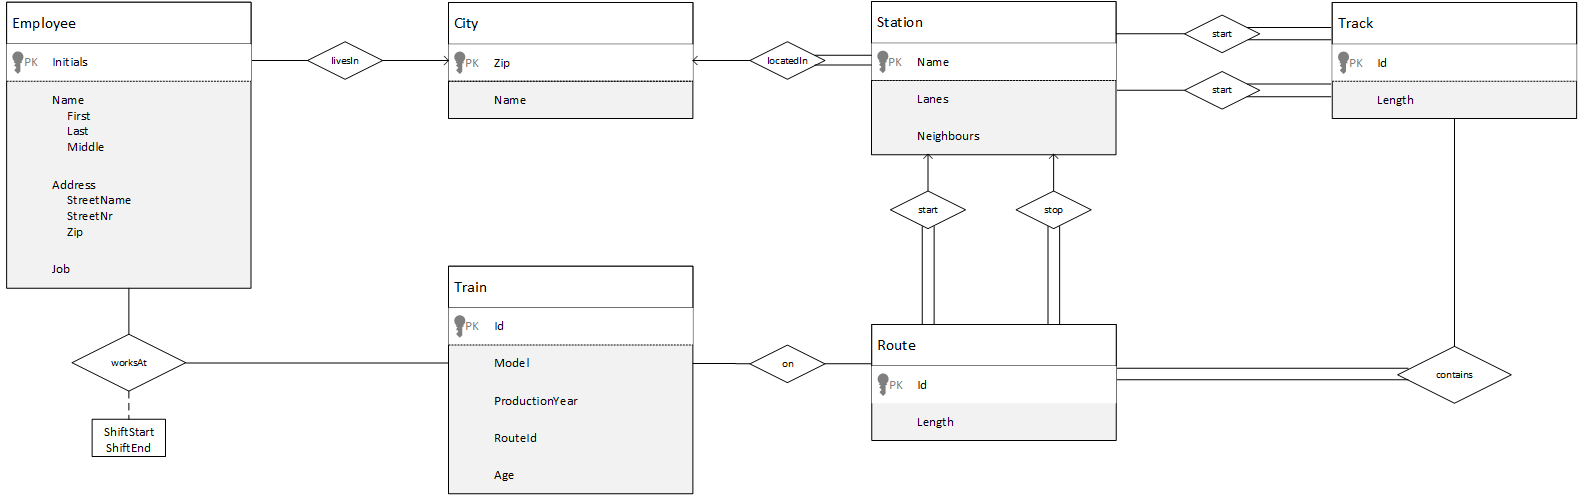
\includegraphics[angle=90,origin=c,width=.4\textwidth]{img/Handwritten_ER}
    \caption{An ER diagram depiction the design of the database}
    \label{fig:ER}
\end{figure}

% Comments on ER diagram supporting the requirements
\newpage
\subsection{SQL Data Manipulation}
When inserting into the empty schema, it is necessary to insert cities as the first thing. Next is stations, followed by tracks, routes, trains, employees, etc. This is because of the relations and their total participation in each other. For example, a track can not exist without having a station in each end.\\
Also, when inserting data into a relation, the values of the insert statement of course has to correspond with the relation design on our ER diagram.\\
An example of inserting cities, would be done by statements like the following:

\begin{figure}[ht!]
    \centering
    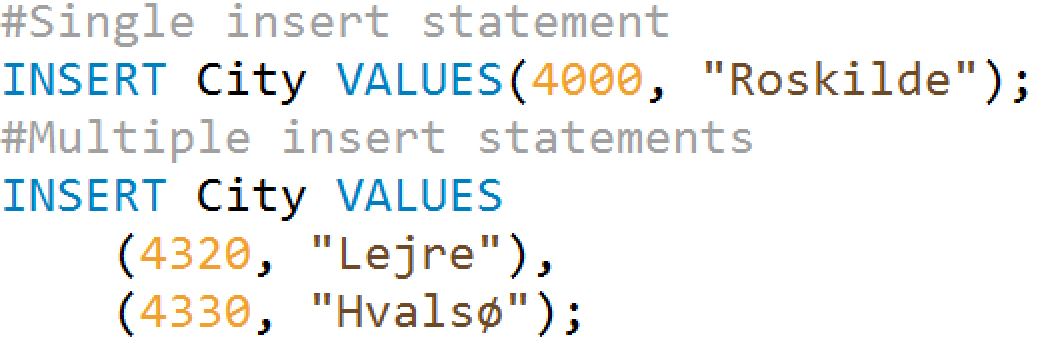
\includegraphics[width=.6\textwidth]{img/INSERT_Statements}
    \caption{SQL INSERT statements for City}
\end{figure}

It is now possible to insert stations located in the existing cities

\begin{figure}[ht!]
    \centering
    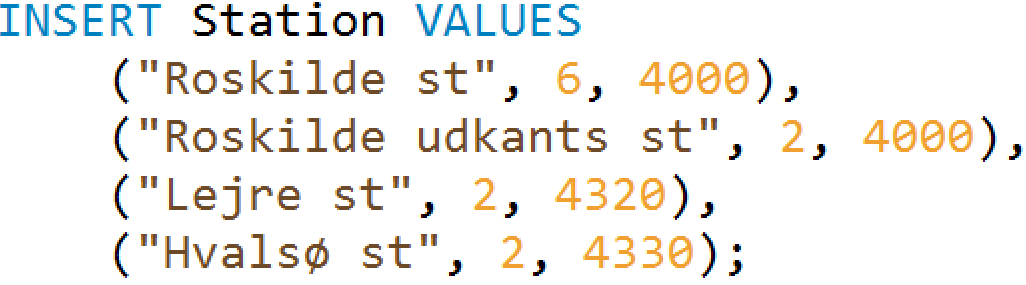
\includegraphics[width=1\textwidth]{img/INSERT_Statement_Station}
    \caption{SQL INSERT statements for Station}
\end{figure}

and then connect these stations with tracks.

\begin{figure}[ht!]
    \centering
    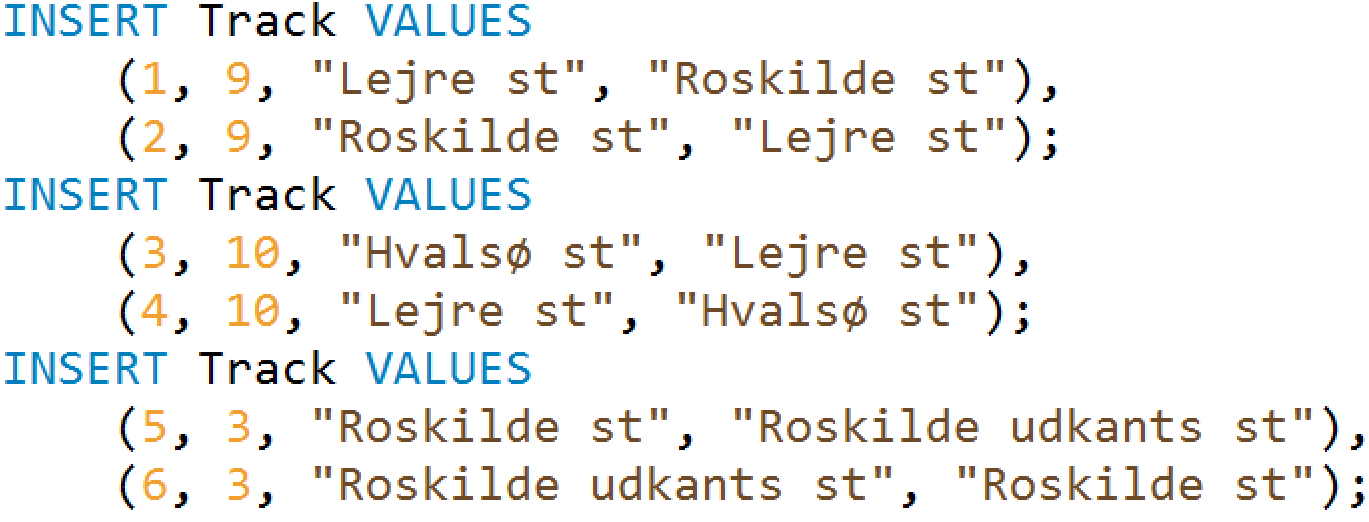
\includegraphics[width=1\textwidth]{img/INSERT_Statements_Track}
    \caption{SQL INSERT statements for Track}
\end{figure}

Finally, we can now insert routes that are composed of existing tracks.

\begin{figure}[ht!]
    \centering
    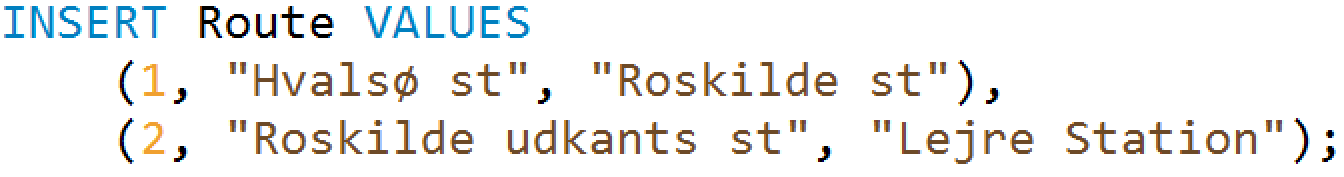
\includegraphics[width=.6\textwidth]{img/INSERT_Statements_Route}
    \caption{SQL INSERT statements for Route}
\end{figure}

When routes have been inserted it is necessary to have a relation containing which tracks each route is composed of. This is the \emph{RouteTracks} relation, which we will insert into now.

\begin{figure}[ht!]
    \centering
    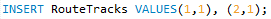
\includegraphics[width=.5\textwidth]{img/INSERT_Statements_RouteTracks}
    \caption{SQL INSERT statements for RouteTracks}
\end{figure}

We are now interested in having trains driving on these existing routes.

\begin{figure}[ht!]
    \centering
    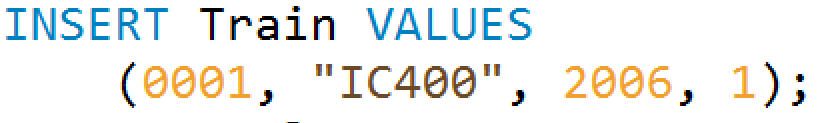
\includegraphics[width=.5\textwidth]{img/INSERT_Statements_Train}
    \caption{SQL INSERT statements for Train}
\end{figure}

However, a train does not have to be on a route. Say, it could be at the workshop, but it is still an existing train.
\newpage
There is of course employees driving and controlling these trains, so lets insert some employees

\begin{figure}[ht!]
    \centering
    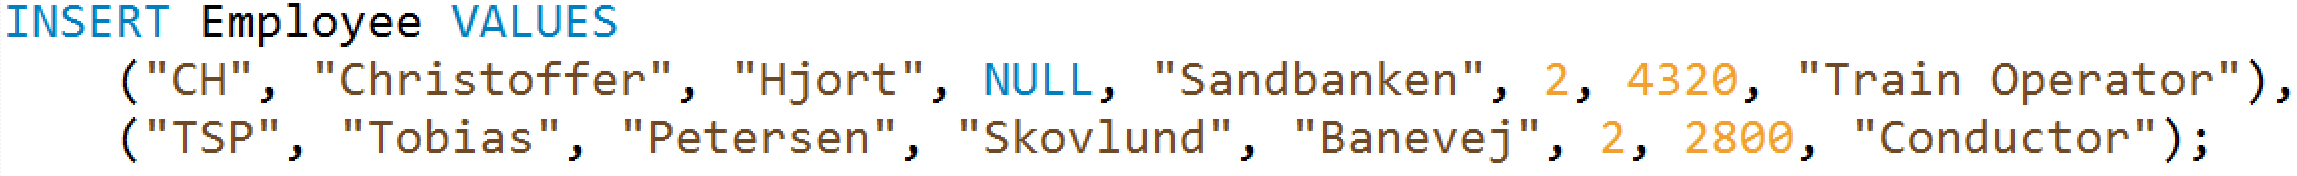
\includegraphics[width=1\textwidth]{img/INSERT_Statements_Employee}
    \caption{SQL INSERT statements for Employee}
\end{figure}

An employee can have a workshift on a train, which is stored as a tuple in the \emph{Shift} relation.

\begin{figure}[ht!]
    \centering
    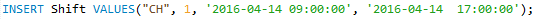
\includegraphics[width=.9\textwidth]{img/INSERT_Statements_Shift}
    \caption{SQL INSERT statements for Shift}
\end{figure}

When deleting tuples or dropping relations, the total participation of the relations comes into play again, just like when inserting into the schema.\\
In the \emph{Train Management} schema, the relations with total participation has been set to \emph{ON DELETE CASCADE}. So, if you were to delete a city which contained stations connected with tracks and routes, it would delete the routes, tracks and stations as well.\\

\begin{figure}[ht!]
    \centering
    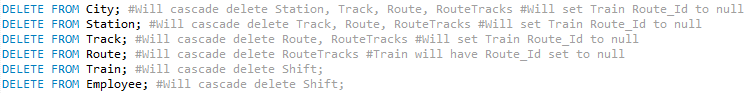
\includegraphics[width=1\textwidth]{img/DELETE_Statements}
    \caption{SQL DELETE statements}
\end{figure}

Not having the relations set to \emph{ON DELETE CASCADE}, the relations would have to be deleted in the correct order, starting from the bottom of the above figure.
\\[12pt]
Updates do not cascade, as the primary keys and foreign keys of relations 
should never need to be changed/updated. ID's should always stay the same, so 
``should'' city names and stations names. If a route were to have its start or 
stop station changed, we would simply insert a new route, rather than updating 
the old.\\
There are still other attributes that are useful to update though, as seen in the examples below.

\begin{figure}[ht!]
    \centering
    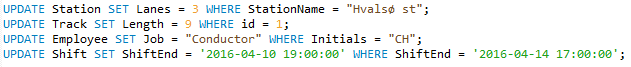
\includegraphics[width=1\textwidth]{img/UPDATE_Statements}
    \caption{SQL UPDATE statements}
\end{figure}
\newpage

\subsection{SQL Programming}
To control the data integrity and make insertion easier and less trivial or calculating attributes, a couple of functions, triggers, procedures, transactions and events have been programmed and implemented.
\\[12pt]
Each station has a specific capacity, that is amount of lanes. And, to make sure that no more tracks are connected to a station than there is capacity, a trigger has been implemented to prevent insertion.

\begin{figure}[ht!]
    \centering
    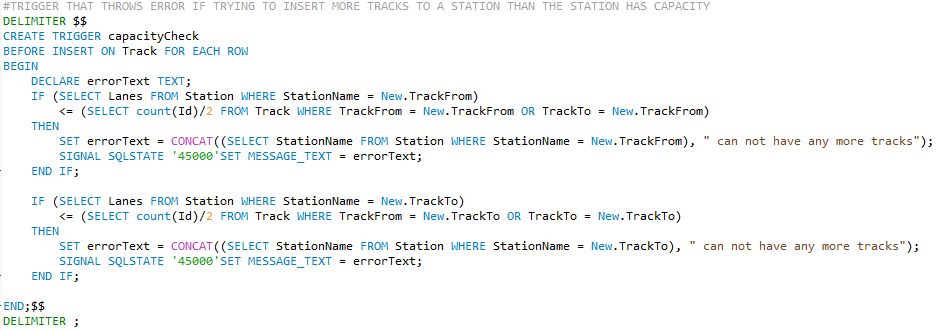
\includegraphics[width=1\textwidth]{img/SQL_TRIGGER}
    \caption{SQL Trigger}
\end{figure}

For example, if Station A has 2 lanes, which is equals to 4 tracks (For each lane there is 1 ingoing track and 1 outgoing), then the trigger would throw an error 1644, and prevent insertion of connecting a fifth track to Station A.

\begin{figure}[ht!]
    \centering
    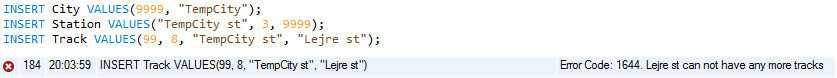
\includegraphics[width=1\textwidth]{img/SQL_TRIGGER_example}
    \caption{SQL Trigger example}
\end{figure}

Lejre st has 2 lanes and already had 4 tracks connected (2 tracks for each connected city), so trying to connect a fifth resulted in an error from the Trigger which triggers \emph{BEFORE INSERT}.

A couple of functions has also been implemented. These are primarily used to calculate dynamic attributes for the relations.\\
This is used calculating the length of a route

\begin{figure}[ht!]
    \centering
    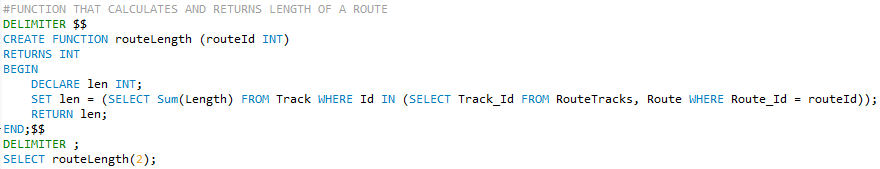
\includegraphics[width=1\textwidth]{img/SQL_FUNCTION_Length}
    \caption{SQL Function for Track Length}
\end{figure}
\newpage

A function for calculating the age of a train.

\begin{figure}[ht!]
    \centering
    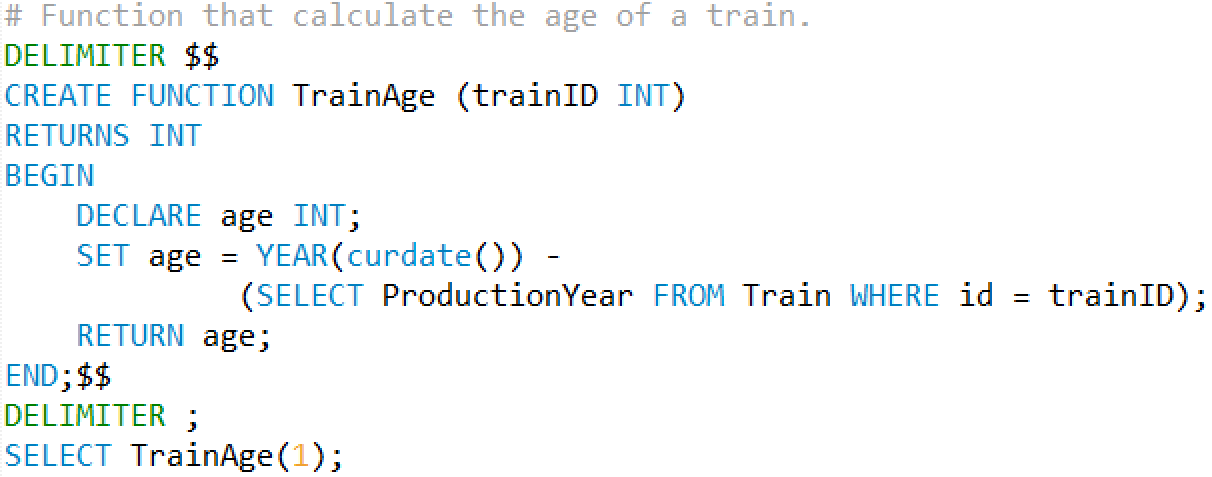
\includegraphics[width=1\textwidth]{img/SQL_FUNCTION_Age}
    \caption{SQL Function for Train Age}
\end{figure}

Next up is the implemented procedures. Some of the procedures only reads from the tables, while other procedures also performs data manipulation.

\begin{figure}[ht!]
    \centering
    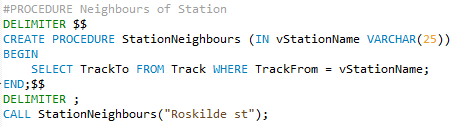
\includegraphics[width=1\textwidth]{img/SQL_PROCEDURE_Neighbours}
    \caption{SQL Procedure for finding Station neighbours}
\end{figure}

\begin{figure}[ht!]
    \centering
    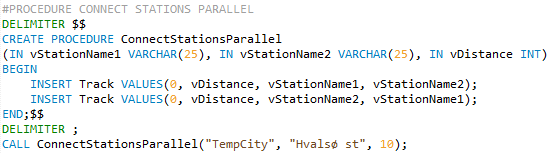
\includegraphics[width=1\textwidth]{img/SQL_PROCEDURE_ConnectParallel}
    \caption{SQL Procedure for connecting stations parallel both ways}
\end{figure}

The procedure inputs 0 to the ID's of the tracks, because our ID's automatically increments from the newest ID.
\newpage
In this last procedure, a transaction has been included. This is to make sure, that the city and station do not get inserted unless it is possible to connect it to the targeted station.

\begin{figure}[ht!]
    \centering
    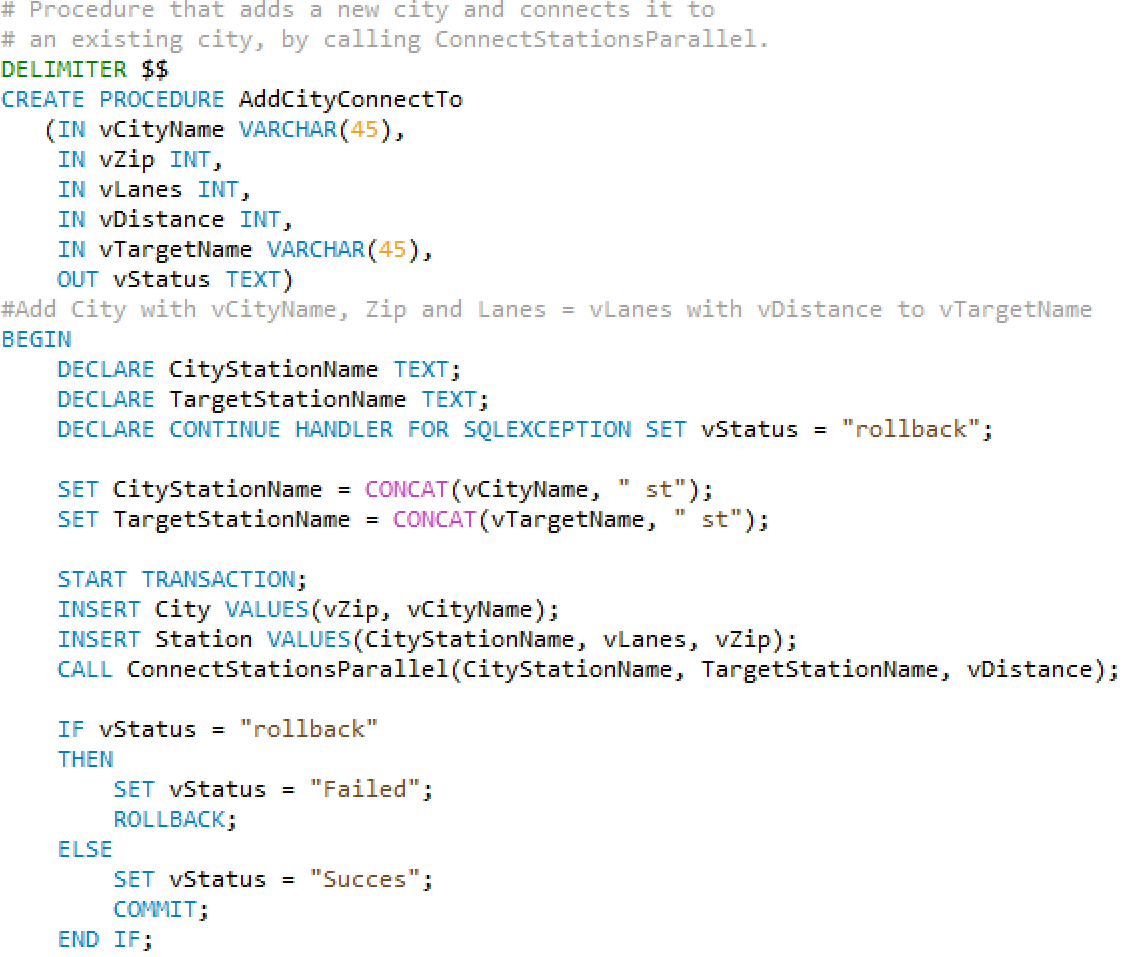
\includegraphics[width=1\textwidth]{img/SQL_PROCEDURE_AddCityConnect}
    \caption{SQL Procedure for connecting new city to target city}
\end{figure}

The procedure adds a new city to the database, creates the main station for the city, and connects it to the specified existing target city, with a specified distance, by adding tracks between them.

\begin{figure}[ht!]
    \centering
    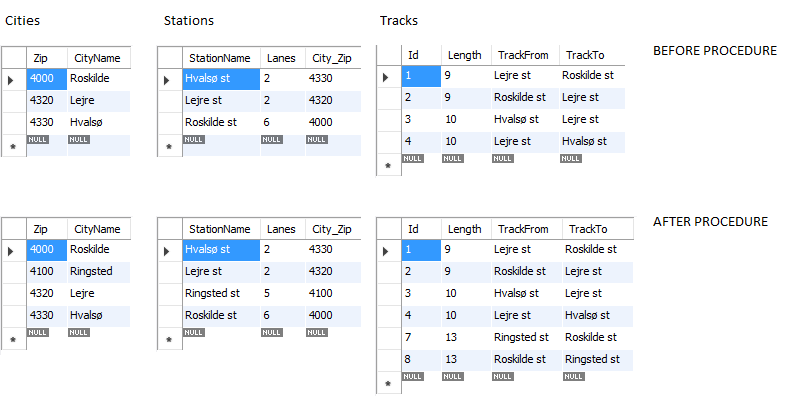
\includegraphics[width=1\textwidth]{img/SQL_PROCEDURE_AddCityConnect_example}
    \caption{Before and after the above procedure}
\end{figure}
\newpage

The only event, is really not a required functionality, as our \emph{Train Management} schema really has no need of events in its current state. 

\begin{figure}[ht!]
    \centering
    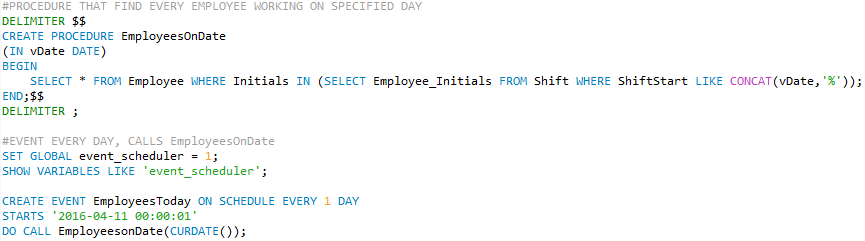
\includegraphics[width=1\textwidth]{img/SQL_EVENT}
    \caption{SQL Event for finding todays employees}
\end{figure}

This event tells who's at work everyday.
The implemented event, is more for general managing, as it is nice to know for each day of the week what employees are at work.